\documentclass[15pt,a5paper,reqno]{article}
\usepackage{hyperref}
\usepackage[warn]{mathtext}
\usepackage[utf8]{inputenc}
\usepackage[T2A]{fontenc}
\usepackage[russian]{babel}
\usepackage{amssymb, amsmath, multicol}
\usepackage{graphicx}
\usepackage[shortcuts,cyremdash]{extdash}
\usepackage{wrapfig}
\usepackage{gensymb}
\usepackage{floatflt}
\usepackage{lipsum}
\usepackage{verbatim}
\usepackage{concmath}
\usepackage{euler}
\usepackage{xcolor}
\usepackage{etoolbox}
\usepackage{fancyhdr}
\usepackage{subfiles}
\usepackage{enumitem}
\usepackage{amsthm}
\usepackage{indentfirst}
\usepackage{import}

\DeclareMathOperator{\sign}{sign}

\RequirePackage[ left     = 1.5cm,
  right    = 1.5cm,
  top      = 2.0cm,
  bottom   = 1.25cm,
  includefoot,
  footskip = 1.25cm ]{geometry}
\setlength    {\parskip}        { .5em plus .15em minus .08em }
%\setlength    {\parindent}      { .0em }
\renewcommand {\baselinestretch}{ 1.07 }

\fancyhf{}

\renewcommand{\footrulewidth}{ .0em }
\fancyfoot[C]{\texttt{\textemdash~\thepage~\textemdash}}

\makeatletter
\patchcmd\l@section{%
  \nobreak\hfil\nobreak
}{%
  \nobreak
  \leaders\hbox{%
    $\m@th \mkern \@dotsep mu\hbox{.}\mkern \@dotsep mu$%
  }%
  \hfill
  \nobreak
}{}{\errmessage{\noexpand\l@section could not be patched}}
\makeatother
\parindent = 1cm % отступ при красной строке⏎
\pagestyle{fancy}    
\renewcommand\qedsymbol{$\blacksquare$}

\newcommand{\when}[2]{
  \left. #1 \right|_{#2} \hspace
}
\renewcommand{\kappa}{\varkappa}
\RequirePackage{caption2}
\renewcommand\captionlabeldelim{}
\newcommand*{\hm}[1]{#1\nobreak\discretionary{}

\DeclareSymbolFont{T2Aletters}{T2A}{cmr}{m}{it}
{\hbox{$\mathsurround=0pt #1$}}{}}
% Цвета для гиперссылок
\definecolor{linkcolor}{HTML}{000000} % цвет ссылок
\definecolor{urlcolor}{HTML}{799B03} % цвет гиперссылок
 
\hypersetup{pdfstartview=FitH,  linkcolor=linkcolor,urlcolor=urlcolor, colorlinks=true}


%\setcounter{secnum[utf8x]depth}{0}

\begin{document}

% НАЧАЛО ТИТУЛЬНОГО ЛИСТА
\begin{center}
  {\small ФЕДЕРАЛЬНОЕ ГОСУДАРСТВЕННОЕ АВТОНОМНОЕ ОБРАЗОВАТЕЛЬНОЕ\\ УЧРЕЖДЕНИЕ ВЫСШЕГО ОБРАЗОВАНИЯ\\ МОСКОВСКИЙ ФИЗИКО-ТЕХНИЧЕСКИЙ ИНСТИТУТ\\ (НАЦИОНАЛЬНЫЙ ИССЛЕДОВАТЕЛЬСКИЙ УНИВЕРСИТЕТ)\\ ФИЗТЕХ-ШКОЛА РАДИОТЕХНИКИ И КОМПЬЮТЕРНЫХ ТЕХНОЛОГИЙ}\\
  \hfill \break
  \hfill \break
  \hfill \break
  \Huge{Работа 2.5.1. \\ Измерение коэффициента поверхностного натяжения жидкости}\\
\end{center}

\hfill \break
\hfill \break
\hfill \break
\hfill \break
\hfill \break
\hfill \break

\begin{flushright}
  \normalsize{Работу выполнил:}\\
  \normalsize{\textbf{Долгов Александр Алексеевич, группа Б01-106}}\\
\end{flushright}

\begin{center}
  \normalsize{\textbf{Долгопрудный, 2022}}
\end{center}

\thispagestyle{empty} % выключаем отображение номера для этой страницы

% КОНЕЦ ТИТУЛЬНОГО ЛИСТА

\newpage
\thispagestyle{plain}
\tableofcontents
\thispagestyle{plain}
\newpage

\section{Аннотация}

    В данной работе измеряется коэффициент поверхностного натяжения дистиллированной воды и определяются полная поверхностная энергия и количество теплоты, необходимое для изотермического образования единицы поверхности жидкости, при различных значениях температуры.
	
\section{Теоретические сведения}

    \textbf{Коэффициент поверхностного натяжения (поверхностное натяжение) жидкости} ($\sigma$, $[\sigma] = \frac{\text{Н}}{\text{м}}$) - работа, которую нужно совершить, чтобы изотермически и квазистатически площадь поверхности жидкости на единицу при сохранении объёма жидкости неизменным.
    
    Из определения поверхностной энергии и первого начала термодинамики получаем, что:
    \begin{equation}
        \delta A_T = -d\Psi_T\ \footnote{Индекс T означает, что величины берутся для изотермического процесса}
    \end{equation}
    
    \noindentСвободную энергию жидкости можно представить в виде:
    \begin{equation}
        \Psi = \Psi_{\text{об}} + \Psi_{\text{пов}},
    \end{equation}
    где $\Psi_{\text{об}}$ - составляющая свободной энергии, пропорциональная объёму (объёмная свободная энергия), $\Psi_{\text{пов}}$ - составляющая свободной энергии, пропорциональная температуре (поверхностная свободная энергия). Таким образом, $\Psi_{\text{пов}} = \sigma\Pi$, где $\Pi$ - площадь поверхности жидкости.
    
    Получим формулу для количества теплоты, которое нужно сообщить плёнке жидкости в изотермическом процессе для изменения площади поверхности на $d\Pi$. В таком процессе поверхность совершат работу $\delta A_T = -\sigma d\Pi$. 
    
    \noindentПо первому началу термодинамики (для данного процесса):
    \begin{equation}
        dU = TdS + \sigma d\Pi
    \end{equation}
    
    \noindentПо определению поверхностной энергии:
    \begin{equation}\label{free energy}
        \Psi = U - TS \Rightarrow d\Psi = dU - TdS - SdT
    \end{equation}
    
    \noindentОтсюда получаем:
    \begin{equation}
        d\Psi = \sigma d\Pi - SdT \Rightarrow S = -\left(\frac{\partial\Psi}{\partial T}\right)_{\Pi}
    \end{equation}
    
    Так как в качестве термодинамической системы рассматривается плёнка жидкости, то 
    \begin{equation}\label{approximation}
        \Psi_{\text{об}} \ll \Psi_{\text{пов}} \Rightarrow \Psi\approx\Psi_{\text{пов}}
    \end{equation}
    Поэтому последнее соотношение принимает вид:
    \begin{equation}\label{entropy}
        S = -\left(\frac{\partial\Psi_{\text{пов}}}{\partial T}\right)_{\Pi}
    \end{equation}
    
    \noindentПодставим \eqref{entropy} в первое уравнение \eqref{free energy} и учтём \eqref{approximation}:
    \begin{equation}
        \Psi_{\text{пов}} = U + T\left(\frac{\partial\Psi_{\text{пов}}}{\partial T}\right)_{\Pi}
    \end{equation}
    
    Так как коэффициент поверхностного натяжения не зависит от площади поверхности жидкости, то $d\Psi_{\text{пов}} = \sigma d\Pi$. Окончательно получаем:
    \begin{equation}\label{inner energy}
        \boxed{U = \Pi\left(\sigma - T\frac{d\sigma}{dT}\right)}
    \end{equation}
    
    В случае проведения над жидкостью изотермического процесса среди всех величин в \eqref{inner energy} изменяется только площадь, а величина в скобках остаётся постоянной. Отсюда, использую первое начало термодинамики, получаем:
    \begin{equation}\label{heat}
        \delta Q = -T\frac{d\sigma}{dT}d\Pi
    \end{equation}
    
    Из \eqref{heat} видно, что величина $q = \frac{\delta Q}{d\Pi}$ в изотермическом процессе является константой. Это есть количество теплоты, которое необходимо сообщить поверхности плёнки для увеличения её площади на единицу. Приведём окончательную формулу:
    \begin{equation}
        \boxed{q = -T\frac{d\sigma}{dT}}
    \end{equation}
    
    \noindentТакже приведём без вывода формулу Лапласа:
    \begin{equation}
        P_{in} - P_{out} = \sigma\left(\frac{1}{R_1} + \frac{1}{R_2}\right),
    \end{equation}
    где $P_{out}$ - давление во внешней среде, $P_{in}$ - давление внутри жидкости $R_1,\ R_2$ - радиусы главных кривизн поверхности жидкости. Для сферической поверхности формула Лапласа принимает вид:
    \begin{equation}\label{Laplas}
        \boxed{P_{in} - P_{out} = \frac{2\sigma}{R}}
    \end{equation}

\section{Экспериментальная установка}

    \noindentСхема экспериментальной установки приведена на рисунке 1.
    
    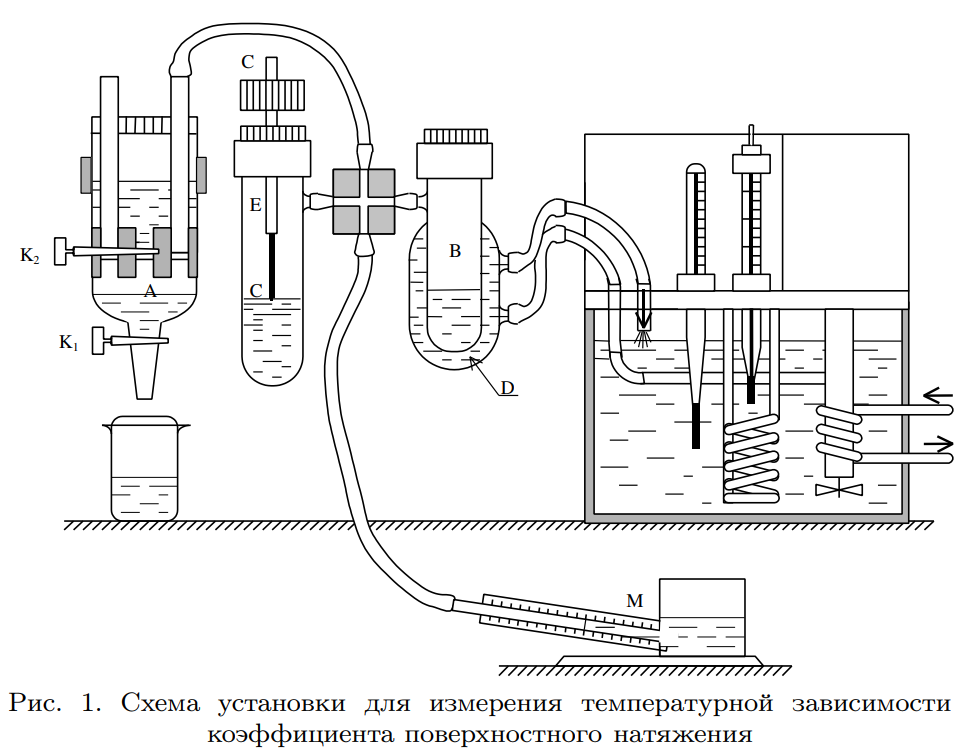
\includegraphics[width = 10cm, height = 7cm]{Рисунок 1.png}
    
    В сосуд \textbf{В} налита исследуемая жидкость (дистиллированная вода), тестовая жидкость (этиловый спирт) налита в сосуд \textbf{Е}. Во время проведения эксперимента обе колбы герметично закрываются пробками. Сосуд, для жидкости в котором проводят измерения, закрывается пробкой, через которую проходит металлическая игла \textbf{С} (другая пробка обычная). Верхний конец иглы сообщён с атмосферой, а нижний погружён в жидкость. При определённой разнице давлений между атмосферой и установкой воздух начнёт проходить через иголку в жидкость (пробулькивание).
    
    Для создания разности давлений в установке предусмотрен аспиратор \textbf{А}, который разделён краном $\textbf{К}_2$ на две области. Та из них, что выше крана заполнена водой. При открытии крана $\textbf{К}_2$ вода поступает в нижнюю область. Разряжения воздуха в установке можно добиться путём открывания крана $\textbf{К}_1$, из которого по каплям вытекает вода. Так как сосуды \textbf{В} и \textbf{С} соединены трубками с нижней областью аспиратора, то при понижении уровня воды объём такого "объединённого сосуда"\ увеличивается, а давление в нём уменьшается. Разность давлений между установкой и атмосферой измеряет я с помощью микроманометра \textbf{М}.
    
    Чтобы температура воды в сосуде \textbf{В} поддерживалась постоянной, рубашка \textbf{D}, окружающая этот сосуд, соединена с термостатом. 
    
\section{Методика измерений}	

    \subsection{Измерения}
    
    Для исключения влияния гидростатического столба жидкости (воздуху приходится через него "пробулькивать") можно разместить иглу \textbf{C} так, чтобы её нижняя часть лишь касалась поверхности жидкости. У данного решения есть ряд проблем, связанных с измерением зависимости коэффициента поверхностного натяжения именно от температуры:
    \begin{enumerate}
        \item Так как игла металлическая, то её теплопроводность выше, чем у жидкости. Поэтому температура нижнего конца иглы будет меньше, чем в объёме жидкости.
        \item Тепловое расширение жидкости в любом случае приводит к образования гидростатического столба внутри иглы
    \end{enumerate}
    
    Для устранения описанных выше проблем можно погрузить иглу как можно глубже, не касаясь дна. Пусть микроманоментр измерил разность давлений $\Delta P_1$, тогда 
    \begin{equation}\label{press}
        \Delta P_1 = \Delta P + \rho gh,
    \end{equation}
    где $\Delta P$ - разность давлений вызванная поверхностным натяжением, $\rho$ - плотность исследуемой жидкости, $h$ - высота гидростатического столба внутри иглы. Так как поперечное сечение иглы постоянно, то величина $\rho h$ отличается от массы на постоянный множитель $\Rightarrow$ величина $\rho h$ практически не изменяется в ходе эксперимента. Эту величину можно измерить двумя способами:
    \begin{enumerate}
        \item Измерим разность давлений $\Delta P'_1$, когда игла лишь касается поверхности жидкости. Затем при той же температуре измерим разность давлений $\Delta P''_1$, когда игла максимально погружена в жидкость. В силу несжимаемости жидкости: 
        
        \begin{equation}\label{rhoh}
            \rho h = \frac{\Delta P''_1 - \Delta P'_1}{g}
        \end{equation}
        \item Во время проведения измерения первым способом можно измерить глубину погружения иглы с помощью линейки. Это можно сделать, измерив, на сколько изменилось расстояние от пробки до верхнего конца иглы при её погружении.
    \end{enumerate}
    
    \subsection{Получение расчётной формулы} 
    
    Шкала микроманометра проградуирована в миллиметрах. Если значение на шкале составляет $p$ мм, то разность давлений, измеренная микроманометром равна
    \[\Delta P_1 = \alpha\frac{\gamma}{\gamma_0}pg\]
    паскалей, где $\alpha$ - постоянная угла наклона, $\gamma$ - текущая плотность спирта в трубке микроманометра, $\gamma$ - плотность спирта, указанная на корпусе микроманометра. В данной работе:
    \[\alpha = 0,2,\ \gamma_0 = 807,5 \frac{\text{кг}}{\text{м}^3},\ \gamma = 803,1 \frac{\text{кг}}{\text{м}^3}\]
    Отношение $\frac{\gamma}{\gamma_0}\approx 0,995\approx 1$, поэтому для данного опыта можно написать:
    \begin{equation}\label{mes}
        \Delta P_1 = 0,2pg,
    \end{equation}
    где $[P_1] = \text{Па}$, $[p] = \text{мм}$.
    
    Так как поперечное сечение иглы имеет форму круга, то поверхность жидкости в игле имеет сферическую или близкую к ней форму. Поэтому для расчётов воспользуемся формулой Лапласа в форме \eqref{Laplas}:
    \[\sigma = \frac{1}{2}R\Delta P = \frac{1}{4}D\Delta P,\]
    где $D$ - диаметр иглы. Далее запишем $\Delta P$, используя формулы \eqref{press} и \eqref{mes}.
    \[\sigma = \frac{1}{4}D(\Delta P_1 - \rho gh) = \frac{1}{4}D(0,2pg - \rho gh)\]
    Окончательно получаем:
    \begin{equation}\label{tension}
        \boxed{\sigma = \frac{1}{4}gD(0,2p - \rho h)}
    \end{equation}
    
\section{Оборудование}
    Диаметр иглы измерялся с помощью микроскопа. Получено значение:
    \[D = 1,15 \pm 0,05\text{ мм}\]
    
    Показания микроманометра и линейки (измерение глубины погружения иглы) измерялись с точностью $0,5\text{ мм}$. 

\section{Обработка полученных результатов}

    \subsection{Глубина погружения иглы}
    Данное измерение состояло из двух серий: сначала игла лишь касалась поверхности спирта, а затем была погружена полностью. Для каждого случая разность давлений измерялась 10 раз. Результаты измерений приведены в таблице 1. Также в этой таблице представлены результаты измерений расстояния от пробки до верхнего конца иглы для каждой из серий.
    
    На основании этих данных усредним значения $\Delta P'_1$ и $\Delta P''_1$ для каждой серии. Значение $\rho h$ найдём по формуле \eqref{rhoh}:

    \noindent Игла лишь касается поверхности спирта:
    \[\langle\Delta P'_1\rangle = 0,2 \cdot 9,81 \cdot 118\text{ Па} = 232\text{ Па}\]
    \[\sigma'_{\text{случ}} = \sqrt{\frac{1}{90}\sum_{i = 1}^{10}(\Delta P'_1 - \langle\Delta P'_1\rangle)} = 0,3\text{ Па}\ \sigma'_{\text{сист}} = 0,2 \cdot 9,81 \cdot 0,5\text{ Па} \approx 1\text {Па}\]
    \[\sigma' = \sqrt{(\sigma'_{\text{случ}})^2 + (\sigma'_{\text{сист}})^2} \approx 1\text{ Па}\]
    
    \noindent Игла максимально погружена в спирт:
    \[\langle\Delta P''_1\rangle = 0,2 \cdot 9,81 \cdot 197,4\text{ Па} = 387\text{ Па}\]
    \[\sigma''_{\text{случ}} = \sqrt{\frac{1}{90}\sum_{i = 1}^{10}(\Delta P''_1 - \langle\Delta P''_1\rangle)} = 0,16\text{ Па};\ \sigma''_{\text{сист}} = 0,2 \cdot 9,81 \cdot 0,5\text{ Па} \approx 1\text {Па}\]
    \[\sigma'' = \sqrt{(\sigma''_{\text{случ}})^2 + (\sigma''_{\text{сист}})^2} \approx 1\text {Па}\]
    
    \noindent Отсюда получаем:
    \[\rho h = \frac{387 - 232}{9,81}\frac{\text{кг}}{\text{м}^2} = 15,8\ \frac{\text{кг}}{\text{м}^2}\]
    \[\sigma_{\rho h} = \frac{1}{g}\sqrt{(\sigma')^2 + (\sigma'')^2} \approx 1,4\ \frac{\text{кг}}{\text{м}^2}\]
    
    \noindentТаким образом: $\rho h = (15,8 \pm 1,4)\text{ Па}$
    
    Используя измеренное расстояние от пробки до верхней части иглы в обеих сериях экспериментов, получаем:
    \[\rho h = 1000\ \frac{\text{кг}}{\text{м}^3} \cdot (22 - 6,5)\text{ мм} = 15,5\ \frac{\text{кг}}{\text{м}^2}\]
    \[\sigma_{\rho h} = 1000\ \frac{\text{кг}}{\text{м}^3} \cdot \sqrt{0,5^2 + 0,5^2}\text{ мм} \approx 0,7\text{ Па}\]
    Таким образом: $\rho h = (15,5 \pm 0,7)\text{ Па}$
    
    Отрезок, на котором лежит граница абсолютной погрешности $\rho h$, найденный вторым способом (измерением расстояния), полностью принадлежит отрезку, найденному первым способом. Поэтому их пересечение - второй отрезок. Таким образом, далее считаем, что 
    \[\rho h = (15,5 \pm 0,7)\text{ Па}\]
    
    \subsection{Поверхностное натяжение}
    Для определения зависимости поверхностного натяжения от температуры было проведено 8 измерений разности давлений при различных значениях температуры. В течение каждого измерения показания с микроманометра снимались в тот момент, когда они практически не отличались для последовательных "пробулькиваний". Таким образом, для каждого измерения получено единственное значение разности давлений. Данные приведены в таблице 2. В таблице также представлены значения коэффициентов поверхностного натяжения, вычисленные по формуле \eqref{tension}, и их погрешности.
    
    Остановимся более подробно на вычислении погрешности. Пусть $\Delta_{\sigma}$, $\Delta_D$, $\Delta_{\rho h}$, $\Delta_p$ - соответственно погрешности коэффициента поверхностного натяжения, диаметра иглы, величины $\rho h$ и показаний микроманометра. Тогда:
    \[\Delta_{\sigma} = \sqrt{\left(\frac{\partial\sigma}{\partial D}\right)^2\Delta_{D}^2 + \left(\frac{\partial\sigma}{\partial p}\right)^2\Delta_{p}^2 + \left(\frac{\partial\sigma}{\partial (\rho h)}\right)^2\Delta_{\rho h}^2}\]

    Из \eqref{tension} получаем:
    \[\frac{\partial\sigma}{\partial D} = \frac{1}{4}g(0,2p - \rho h);\ \frac{\partial\sigma}{\partial p} = \frac{1}{20}gD;\  \frac{\partial\sigma}{\partial (\rho h)} = -\frac{1}{4}gD\]
    Откуда:
    \[\Delta_{\sigma} = \frac{1}{4}g\sqrt{(0,2p - \rho h)^2\Delta_{D}^2 + D^2\left(\frac{\Delta_{p}^2}{25} + \Delta_{\rho h}^2\right)}\]
    \textit{Замечание:} в данную формулу $g$ подставляется численно, $p$ и $D$ - в миллиметрах, $\rho h$ - в $\frac{\text{кг}}{\text{м}^2}$; размерности погрешностей соответствуют размерности самих величин; размерность результата - $\frac{\text{мН}}{\text{м}}$.
    
    Зависимость $\sigma(T)$, построенная согласно таблице 1, отражена на графике 1. По методу наименьших квадратов получены коэффициенты, описывающие наилучшую прямую, проходящую через экспериментальные точки. Если $\sigma(T) = kT + b$, то
    \[k = (-0,159 \pm 0,007)\frac{\text{мН}}{\text{м}\cdot\text{К}}\]
    \[b = (115 \pm 2)\ \frac{\text{мН}}{\text{м}}\]
    
    Графики зависимостей теплоты образования единицы поверхности и внутренней энергии поверхности от температуры также приведены в приложении (в качестве $\frac{d\sigma}{dT}$ берётся найденный из МНК коэффициент $k$).

\section{Вывод}

    В ходе данной работы была измерена температурная зависимость коэффициента поверхностного натяжения воды. Полученное значение с точностью до найденное абсолютной погрешности совпадает с табличными значениями (например, задача 12.9 из "Сборник задач по общему курсу физики. Ч. 1 / под ред. В.А. Овчинкина 4-е изд., испр. - М.: Физматкнига, 2016. - 560с.").
    
    Стоит, однако, заметить, что значения самого коэффициента поверхностного натяжения не совпадают с табличными в пределах найденных погрешностей (в качестве табличных данный рассматривалось описание данной работы). Тем не менее, можно проследить закономерность, что полученные результаты отличаются от табличных примерно на одну и ту же величину (меньше на $\approx 4\frac{\text{мН}}{\text{м}}$). Такая погрешность, очевидно, систематическая. Поэтому её можно объяснить либо ошибкой экспериментатора, либо тем, что не было учтено влияние некоего внешнего фактора. Этим же объяснятся довольно странный характер графика 4.

\newpage
\section{Приложения}

    \subsection{Таблица 1. Измерение глубины погружения нити}
    \begin{center}
        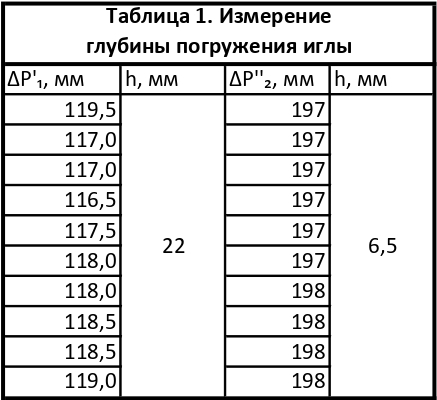
\includegraphics{Таблица 1.jpg}
    \end{center}
    
    \subsection{Таблица 2. Поверхностное натяжение}
    \begin{center}
        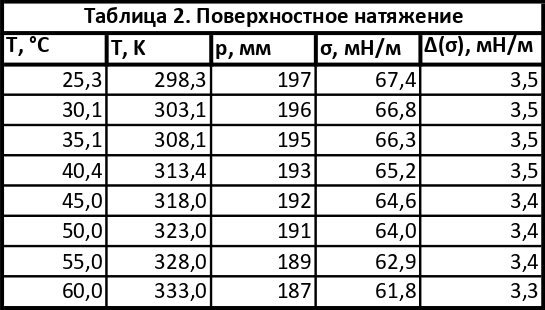
\includegraphics{Таблица 2.jpg}
    \end{center}
    
    \subsection{График 1. Температурная зависимость поверхностного натяжения}
    \begin{center}
        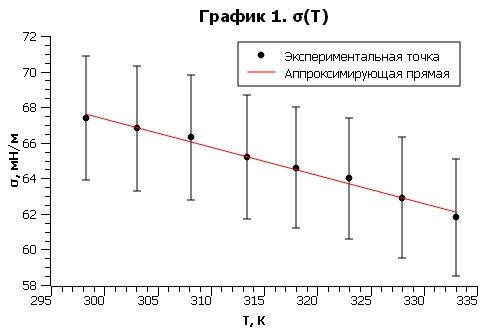
\includegraphics[width = 9cm]{График 1.jpg}
    \end{center}
    
    \subsection{График 2. Теплота образования единицы поверхности}
    \begin{center}
        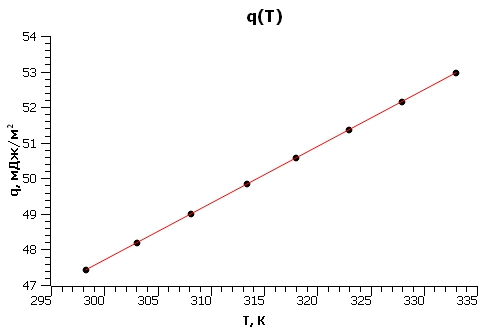
\includegraphics[width = 9cm]{График 2.jpg}
    \end{center}
    
    \subsection{График 3. Удельная внутренняя энергия поверхности}
    \begin{center}
        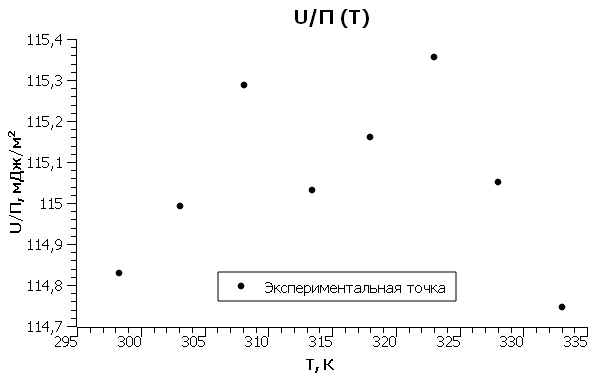
\includegraphics[width = 9cm]{График 3.jpg}
    \end{center}

\end{document}